\documentclass[tikz,border=6pt]{standalone}
\usepackage{amsmath,amssymb}
\usepackage{xcolor}
\definecolor{accent}{HTML}{A13D2C}
\definecolor{accent2}{HTML}{2B5F6B}
\definecolor{muted}{HTML}{5A564F}
\definecolor{linecol}{HTML}{D8D2C4}
\usetikzlibrary{arrows.meta}
% Schematic transit of an Earth across a Sun-like star (code/ch7/01_transit_snr.awk).
% Depth (R_E/R_S)^2 = 84 ppm, duration 12.98 h (central crossing), ingress 0.12 h (= R_E/R_S x 13 h).
% Bands: +-30 ppm (Kepler's measured precision over 6.5 h, 12th magnitude) and
%        +-10 ppm (shot noise over 6.5 h from the estimate in the text). x in hours, y in ppm.
\usepackage[T1]{fontenc}\usepackage{newpxtext,newpxmath}  % same fonts as the notes
\begin{document}
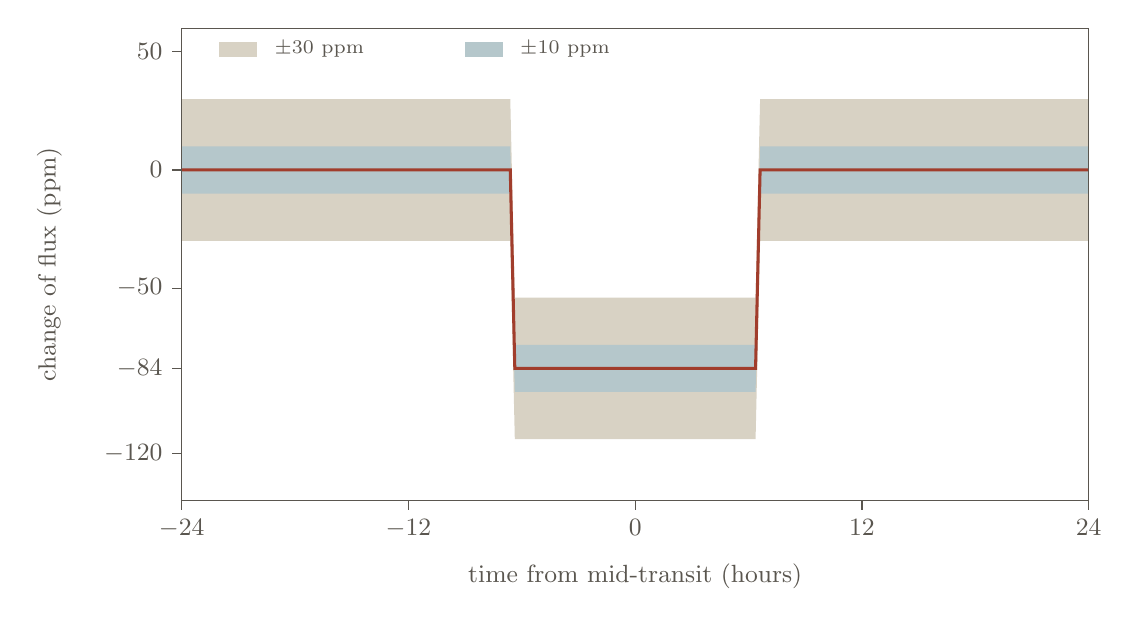
\begin{tikzpicture}[x=0.24cm, y=0.03cm, >={Stealth[length=2.4mm]}]
  \def\d{84}\def\h{6.49}\def\g{6.61}   % depth, half-duration at mid-ingress +-0.06 h
  \def\hi{6.37}
  % bands: model +- sigma
  \foreach \s/\c in {30/linecol, 10/accent2!35} {
    \fill[\c] (-24,\s) -- (-\g,\s) -- (-\hi,-\d+\s) -- (\hi,-\d+\s) -- (\g,\s) -- (24,\s)
              -- (24,-\s) -- (\g,-\s) -- (\hi,-\d-\s) -- (-\hi,-\d-\s) -- (-\g,-\s) -- (-24,-\s) -- cycle;
  }
  % model
  \draw[accent, line width=1.1pt] (-24,0) -- (-\g,0) -- (-\hi,-\d) -- (\hi,-\d) -- (\g,0) -- (24,0);
  % axes
  \draw[muted] (-24,-140) rectangle (24,60);
  \foreach \t in {-24,-12,0,12,24} \draw[muted] (\t,-140) -- (\t,-144) node[below] {\small $\t$};
  \node[muted] at (0,-172) {\small time from mid-transit (hours)};
  \foreach \y in {0,-84} \draw[muted] (-24,\y) -- (-24.5,\y) node[left] {\small $\y$};
  \foreach \y in {50,-50,-120} \draw[muted] (-24,\y) -- (-24.5,\y) node[left] {\small $\y$};
  \node[muted, rotate=90] at (-31,-40) {\small change of flux (ppm)};
  % key
  \fill[linecol] (-22,48) rectangle (-20,54); \node[muted, right] at (-19.6,51) {\scriptsize $\pm30$ ppm};
  \fill[accent2!35] (-9,48) rectangle (-7,54); \node[muted, right] at (-6.6,51) {\scriptsize $\pm10$ ppm};
\end{tikzpicture}
\end{document}
